\section{Open Source Software \textbf{StrainTool v1.0}}
 
\graphicspath{{Chapter2/Figs/}}

\begin{frame}
  \frametitle{Open Source Software \textbf{StrainTool v1.0}}
  \framesubtitle{\citep{anastasiou2019}}
  \label{ch2:straintool}
  
  \begin{columns}
    \begin{column}{0.5\textwidth}
      StrainTool has three basic components:
      \begin{itemize}
        \item \textbf{pystrain:} A python package.
        \item \textbf{StrainTensor.py:} the main executable.
        \item A list of shell scripts to plot results from StrainTensor.py
      \end{itemize}
    \end{column}
    \begin{column}{0.5\textwidth}
      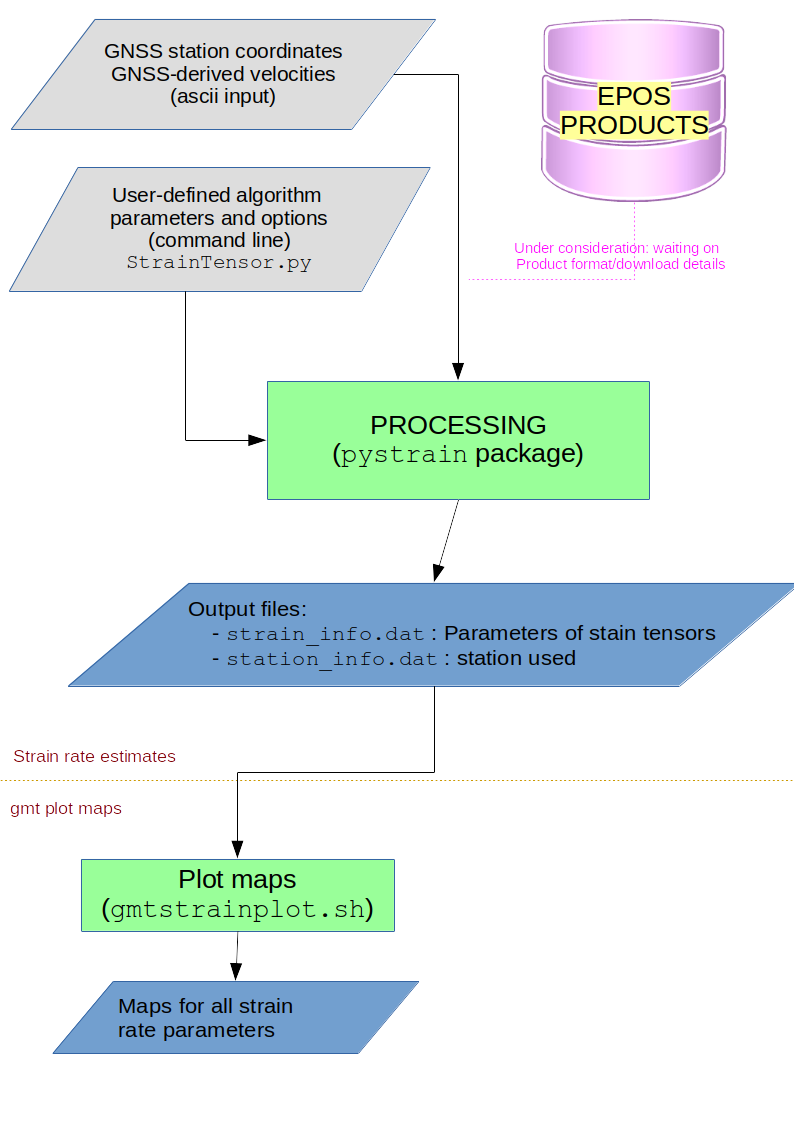
\includegraphics[width=0.8\textwidth]{StrainTool-flowchart.png} 
    \end{column}
  \end{columns}
\end{frame}
\note{}


\begin{frame}
  \frametitle{Python Package \texttt{pystrain}}
  \framesubtitle{}
  \label{ch2:}
  
  \texttt{pystrain} the core part of the project.
  
  Python functions and classes, enable computation of strain tensor.
  
  The package includes:
  \begin{itemize}
    \item \texttt{iotools}: input/output classes to parse ASCII files.
    \item \texttt{geodesy}: functions for basic geodetic calculations.
    \item \texttt{grid.py}: a simple grid generator
    \item \texttt{strain.py}: main class and necessary functions for estimation of strain  tensor parameters
  \end{itemize}
  
  

\end{frame}
\note{}


\begin{frame}
 \frametitle{Estimate strain tensor parameters}
 \framesubtitle{}
 \label{ch2:}
 
 Strain tensor parameters estimated (or calculated) by solving for the system:
 
 \[
  \begin{bmatrix}
    V_{x,S_1} \\ 
    V_{y,S_1} \\ 
    \cdots \\ 
    V_{x,S_n} \\ 
    V_{y,S_n} \\ 
  \end{bmatrix}
  =
  \begin{bmatrix}
    1 & 0 & \Delta_{y_1}  & \Delta_{x_1} & \Delta_{y_1} & 0 \\
    0 & 1 & -\Delta_{x_1} &  0           & \Delta_{x_1} & \Delta_{y_1} \\
    \cdots & \cdots & \cdots & \cdots & \cdots & \cdots \\
    1 & 0 & \Delta_{y_n}  & \Delta_{x_n} & \Delta_{y_n} & 0 \\
    0 & 1 & -\Delta_{x_n} &  0           & \Delta_{x_n} & \Delta_{y_n} \\
  \end{bmatrix}
  \begin{bmatrix}
    U_{x} \\ 
    U_{y} \\ 
    \omega \\ 
    \tau_{x} \\ 
    \tau_{xy} \\ 
    \tau_{y} \\ 
  \end{bmatrix}
  \]
  
  $V_{x,S_1}, V_{y,S_1}$ : North-east velocity components for station $S_1$
  
  $\Delta_{x_i}, \Delta_{y_i}$ : Displacement components between station i and cell center.
  
  $ U_{x},  U_{y} $ : Translation components.
  
  $\omega$ : Total solid body rotation.
  
  $ \tau_{x}, \tau_{xy}, \tau_{y} $ : Horizontal strain components.
  
  A minimum of three stations is required to compute the parameters.
  
%   \textcolor{red}{explain all parameters}
  

\end{frame}
\note{}

\begin{frame}
 \frametitle{Estimate strain tensor parameters}
 \framesubtitle{}
 \label{ch2:}
 
 Assuming that there is variance information for the station velocities (and a Gaussian distribution), we can include the covariance matrix C  of the velocity data in the system. In the simplest case, C is a diagonal matrix, with the velocity component standard deviations as its elements.
 
 \[
 C = \sigma_{0}^{2} 
 \begin{bmatrix}
 (\frac{1}{\sigma_{V_{x_{1}S_{1}}}})^{2} & 0 & 0  & ... & 0\\
 0 & (\frac{1}{\sigma_{V_{y_{1}S_{1}}}})^{2} & 0  & ... & 0\\
 0 & 0 & ({\frac{1}{\sigma_{V_{x_{2}S_{2}}}}})^{2} & ... & 0\\
 ... &  ... & ... & ... & ...\\
 0 & 0 & 0 & ... & (\frac{1}{\sigma_{V_{y_{i}S_{i}}}})^{2}\\
 \end{bmatrix}
 \]

\end{frame}
\note{}


\begin{frame}
 \frametitle{Shen Algorithm}
 \framesubtitle{\citep{Shen2015}}
 \label{ch2:}
 
 Shen et al. 2015, propose a more elaborate approach.
 
 The weighting function
 
 \[ G_{i} = L_{i} Z_{i}  \]
 
 $ L_{i} $ : distance-dependent weighting
 
 $ Z_{i} $ : spatial weighting
 
 The final covariance matrix $ C_{i} = C_{i}G_{i}^{-1} $

\end{frame}
\note{}

\begin{frame}
  \frametitle{Shen Algorithm}
  \framesubtitle{Optimal smoothing parameter D}
  \label{ch2:}
 
  Smoothing coefficient D needed to actually compute the distance-dependent weights  $L_{i}$.
 
  \begin{itemize}
    \item Either pass in the parameter value as a command line option, or
    \item search for an optimal D value, given the range Dmin, Dmax, Dstep, and the limit value W
  \end{itemize}
  
  Searching for an optimal D value
  
  \begin{enumerate}
    \item If a Gaussian approach is selected, then Lmax = 2.15D (in km), while for the quadratic approach Lmax = 10D (in km).
    \item Compute distance-dependent and spatial weights $ L_{i} $ and $ Z_{i} $ respectively, for every station
    \item compute the sum $ W = 2\sum Z_{i} L_{i} $.
    \item repeat the process for the next D value if absolute value W is smaller than Wt, else current D value is optimal.
  \end{enumerate}
 
 

\end{frame}
\note{}

\begin{frame}
  \frametitle{Shen Algorithm}
  \framesubtitle{Distance-dependent weighting}
  \label{ch2:}
  \vskip -.5cm
  \begin{center}
  Weighting for strain. parameter D = 50
    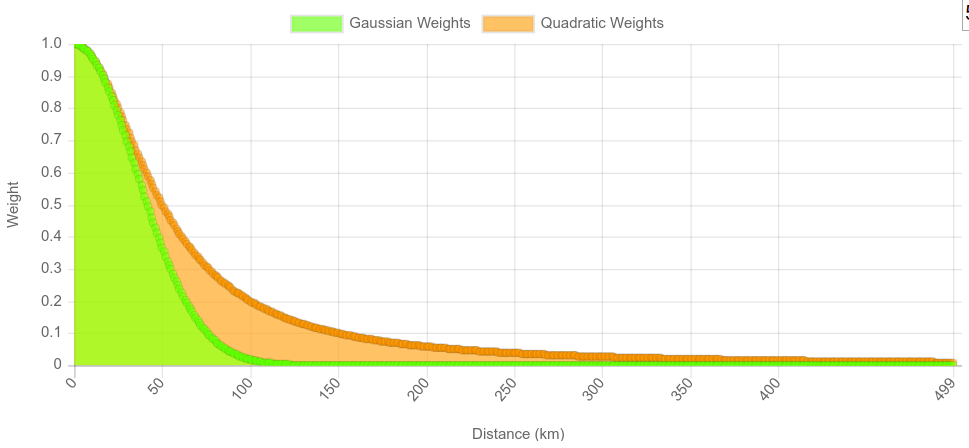
\includegraphics[width=0.9\textwidth]{w_doptimal.png} 
  \end{center}
  Gaussian: $L_i = exp(-\Delta R^2/D^2) $ 
  
  Quadratic: $ L_i = 1/(1 + \Delta R^2/D^2) $
 
\end{frame}
\note{}

\begin{frame}
  \frametitle{Shen Algorithm}
  \framesubtitle{Spatial weights}
  \label{ch2:}
  
   
  \begin{center}
    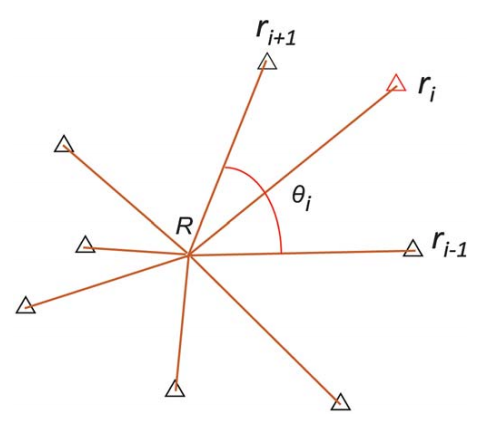
\includegraphics[width=0.5\textwidth]{shen_spatial.png} 
    
    \citep{Shen2015}
  \end{center}
  
  The azimuth span $\theta_i$ of geodetic data point $r_i$ relative to interpolation site R. Triangles denote locations of geodetic data points near the interpolation site R.
  
\end{frame}
\note{}

\begin{frame}
  \frametitle{Veis Algorithm}
  \framesubtitle{\citep{Veis1992}}
  \label{ch2:}
  
  The region is split into delaunay triangles at the barycenter of which a strain tensor is computed.
  
  This approach uses only three points to calculate tensor parameters
  
  \textbf{Assumptions:}
  \begin{itemize}
    \item 2-dimensional deformation of earth's crust in time
    \item Crust is considered a thin deformable shell on a spherical earth
    \item Mapping distortions are ignored for regions with radius of less than 5\textsuperscript{o}
    \item Time (earthquakes) or space (faults) discontinuities are not included in the calculation
  \end{itemize}
\end{frame}
\note{}

\begin{frame}
  \frametitle{Strain Tensor parameters}
  \framesubtitle{}
  \label{ch2:}
  \begin{center}
  \begin{tabular}{l l}
  \toprule
    Parameter & Formula\\
  \midrule
    Maximum shear strain & $ \tau_{max}= \sqrt{ {\tau_{xy}}^2 + {e_{diff}}^2 } $ \\
    Extension & $ e_{max}  = e_{mean} + \tau_{max} $ \\
    Compression & $ e_{min}  = e_{mean} - \tau_{max} $ \\
    Azimouth of $e_{max}$& $ Az_{e_{max}}  = 90 + \frac{-atan2(\tau_{xy}, e_{diff})}{2} $ \\ 
    Dilatation & $ dil = \tau_{x} + \tau_{y} $ \\
    Second Invariand & $ 2nd\_inv = \sqrt{ {\tau_{x}}^2 + {\tau_{y}}^2 + 2{\tau_{xy}}^2  }$\\
  \bottomrule
% $$ Az_{e_{max}}  = 90 + \frac{-atan2(\tau_{xy}, e_{diff})}{2} $$ & $$ dilatation = \tau_{x} + \tau_{y} $$ & $$ second invariant = \sqrt{ {\tau_{x}}^2 + {\tau_{y}}^2 + 2{\tau_{xy}}^2  }$$

  \end{tabular}

  \vskip .3cm
  where,

  \begin{tabular}{c c}
  $ e_{mean} = \frac{\tau_{x}+\tau_{y}}{2} $ & $ e_{diff} = \frac{\tau_{x}-\tau_{y}}{2} $
  \end{tabular}
  \end{center}
%   \textcolor{red}{TODO: make a table with param and math equation}
\end{frame}
\note{}


%\begin{frame}
%   \frametitle{}
%   \framesubtitle{}
%   \label{ch2:}

%\end{frame}
%\note{}
